\documentclass[draftclsnofoot,onecolumn]{IEEEtran}

\usepackage{amsmath,amsthm,amssymb}
\usepackage{graphicx}
\graphicspath{{/home/jingle/figures/}} %path to graphs
\usepackage{subfigure}

\usepackage{url}
\usepackage{cite}

% correct bad hyphenation here
\hyphenation{op-tical net-works semi-conduc-tor}

\begin{document}

\title{Traf: A Camera Based System for Traffic Flow Analysis}
\maketitle
\author{fsb}

\begin{abstract}
As the traffic jam is becoming a serious issue of urban life, collecting traffic parameters for traffic distribution is important and critical.
In this paper, we present a camera based system(Traf) to count automotive vehicles for traffic flow analysis use. The system employs the method of background subtraction by comparing differences between foreground and background.The subtraction result is utilized to identify the position and the shape of vehicles. After unification and pre-treated. The background model is initialed by averaging first 50 frames, and adapted to environment change by introducing an adapting parameter $\lambda$. Compared to state-of-art method, it is more robust, adaptive and economical.

\end{abstract}


%--------------------------------------------------------------------------------
% what and why ?
\section{Introduction}
  With the development of economy, automobile vehicle number is increasing sharply, which brings many traffic jams and increases traffic management cost\cite{sugiyama2008traffic}. One of the most feasible ways to solve these problems is to gather the traffic parameters effectively and distribute the resources of road reasonably\cite{timotheou2015distributed,ni2013rgbd}. The video image based algorithm utilizes computer vision technology\cite{yang2015construction} and cyber physical system, providing an efficient and economical solution towards this issue.

	Different from most rest methods, video image is capable to provide rich information, and it is easy to deploy to varies environment.Besides, the collected information is convenient to store and share, making it possible for traffic monitor, accident analysis and so on \cite{zaccaro2015assessing}. What's more, video based method is friendly for further upgrading. While these advantages are hard to achieve by ultrasonic\cite{jo2014traffic},infrared\cite{harrison2014cognitive} or magnetic performance\cite{ma2016distribution}.

	Currently, there are lots of cameras on the road for traffic monitor, which can hence provide rich original video sources. Lots of methods for moving object recognition and tracking in the intelligent traffic monitoring system was proposed, like frame subtraction \cite{singla2014motion}, but its accuracy is questionable due to the overlapping. Our system is designed to work on the video collected by cameras on the road, and we employed background subtraction algorithm \cite{sobral2014comprehensive} which is efficient and reliable.
	
%================================================================================

% how?

	%============================================================================
\section{System Overview}
	The system consists of 3 main modules, video collector, vehicle counter and flow analyzer as Fig \ref{fig:sysDiagram}. Video collector is designed to collect the original video sources and transform them into a unified format for further use. Flow analyzer is designed to calculate the result and provide suggestion for traffic use. The vehicle counter is the core module of the system, which is further divided into 2 steps as, detector and tracker. 	
	\begin{figure}[!ht]
	\centering
	\subfigure{
	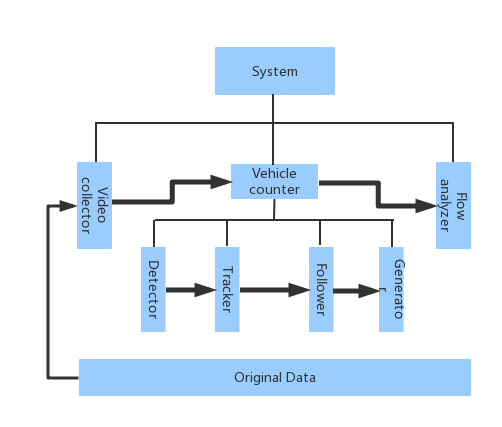
\includegraphics[width=0.45\linewidth]{diagram1.png}}
	\subfigure{
	\includegraphics[width=0.45\linewidth]{diagram2.png} 
	}
	\caption{System diagram:Video collector - Vehicle counter - Flow analyzer}
	\label{fig:sysDiagram}
	\end{figure}
	
	
	%============================================================================
	\section{Background Subtraction}
	As the monitoring camera is deployed with a fixed position, videos collected from this kind of devices would have a stable background. And the automobile vehicles forms the foreground motions. Hence, content of each frame image contains two parts, foreground and background. To detect the vehicles, we utilize background subtraction method, which can be described as:
	\begin{equation}
	F = I  - B
	\label{eq:backgroundSubtraction}
	\end{equation}
	Where $I$ is derived from frame image, $B$ is the corresponding background, and $F$ is hence the detected foreground.
	
	Frame images from video usually have more than one channel, and they may vary from different types and sizes. This makes it hard or impossible for directing subtraction calculation. Hence, we introduce a collector module to unify the original frame images, as Fig.\ref{fig:unifyDiagram}
	\begin{figure}[!h]
	\centering
%	\subfigure[Original frame image]{
%	\includegraphics[width=0.22\linewidth]{frameImg.jpg}}
	\subfigure[I:image frame]{
	\includegraphics[width=0.32\linewidth]{frameImgGry.jpg}}
	\subfigure[B:background model]{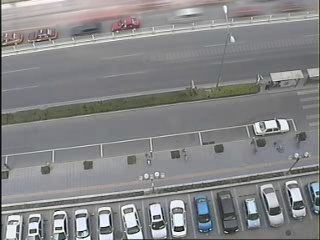
\includegraphics[width=0.32\linewidth]{InitBackgroudFile.jpg}}	
	\subfigure[F:foreground image ]{
	\includegraphics[width=0.32\linewidth]{rawMask.jpg} }
	\caption{Unifying frame image:transform the original image to 8 bits unsigned char with single channel}
	\label{fig:unifyDiagram}
	\end{figure}
	
	After unifying operation, we do background subtraction, and get the foreground image $F$ as Eq.\ref{eq:backgroundSubtraction}. $F$ is mainly consisted of 2 area, the black and the gray. They stands for the background and the foreground separately. However, the gray parts is distributed all the image, making it hard for automobile vehicle detection. Ideally, the gray area of $F$ should gather together as an island. But due to camera performance, environment disturbance and so on, the image carries noise. Even worse,some parts of automobile vehicle may have coincident color with the background overlapping, this would results in gabs and separations.
	\begin{equation}
	  mask=sign(v)=\left\{
	   \begin{aligned}
	   	1, v \geq \delta \\
	   	0, v < \delta \\
	   \end{aligned}
	   \right.
	   \label{eq:foreMask}
	\end{equation}		
	To solve the problem above, we take following strategies as Fig.\ref{fig:preDetection}. First, we employs a Guassian filter with 4*4 size window to reduce noise. Second, we transform the result into binary image with Eq.\ref{eq:foreMask}, the result $Mask$ may consists of several neighbor areas. To make it a nice mask for describing automobile vehicles' shape and position, we employed dilation. Finally, we applied erosion for a better result. 
%	\begin{figure}[!h]
%	\centering
%	\includegraphics[width=0.45\linewidth]{diagram2.png} 
%	\caption{Diagram:Frame image pre-Detection diagram}
%	\label{fig:preDetection}
%	\end{figure}
	
	\begin{figure}[!h]
	\subfigure[Filter Guassian noise]{
	\includegraphics[width=0.22\linewidth]{guassian.jpg} }
	\subfigure[Binary image]{
	\includegraphics[width=0.22\linewidth]{binary.jpg} }
	\subfigure[Dilation]{
	\includegraphics[width=0.22\linewidth]{dilation.jpg} }
	\subfigure[Erosion]{
	\includegraphics[width=0.22\linewidth]{erosion.jpg} }
	\centering
	\caption{Guassian Filter - Binary Image - Dilation - Erosion}
	\label{fig:preDetection}
	\end{figure}
	
	After preview operations, $Mask$ becomes a binary image consists of white islands and black background. The white symbolizes vehicle cars within foreground, and we detect the motion by counting the contour of the island. Considering the size and the shape of a automobile vehicle, it's obviously that islands with small area should be expelled. Then we track the detected motion with Kalma-filter, hence we record the vehicle exactly once for appearing in the view.

\section{Background Model}

One novel point of our system is the background model. As frame images consists of two parts, foreground and background. If there were no automobile vehicles within the frame image, the background is hence equal to the frame image. But this is not always the case, as the automobile vehicles are running on the road from time to time. Even worse, background may change due to light, wind and so on. So a steady background model is essential to the robustness of the system.
	Traf first builds the initial background model by averaging first 50 frame images. The result is shown as \ref{fig:background}
	\begin{figure}
	\subfigure[background in color]{\includegraphics[width=0.32\linewidth]{realBackgroundFile.jpg}}
	\subfigure[background in gray]{\includegraphics[width=0.32\linewidth]{grayBackgroundFile.jpg}}
	\subfigure[background model]{\includegraphics[width=0.32\linewidth]{initBackgroundFile.jpg}}
	\label{fig:background}
	\caption{Background constructing and updating}
	\end{figure}
	
	To adapt to environment change, Traf employs an adaptive parameter $\lambda$ as equation \ref{eq:adaption}.
	\begin{equation}
	M_{t} = (1-\lambda)M_{t-1} + \lambda B_{t}
	\label{eq:adaption}
	\end{equation}
	where $M_t$ and $M_{t-1}$ are the background model at time $t$ and $t-1$, $B_{t}$ is the background derived from frame image at time $t$.
	\begin{eqnarray}	
	F_{t}=&I_{t} - M_{t-1}	\\
	B_{t}=&y(F_{t})*M_{t-1}+(1-y(F_{t}))I_{t}
	\end{eqnarray}
Item $B_{t}$ is built from the mask of foreground and background model at time $t$. The mask is derived from a sign function as:
	\begin{equation}
	  y=sign(F)=\left\{
	   \begin{aligned}
	   	1, F \geq \epsilon \\
	   	0, F < \epsilon \\
	   \end{aligned}
	   \right.
	\end{equation}			

	
% compare and check	

\section{Result}



\section{Conclusion}

\bibliographystyle{plain}
\bibliography{fuck}

\end{document}